
\noindent\begin{minipage}{\textwidth}
    \begin{table}[H]
        \centering
        \caption{Hiperparâmetros e Resultados do Melhor Modelo - swin\_v1\_AB\_opt\_aug}
        \vspace{0.2cm}
        \resizebox{\textwidth}{!}{%
            \begin{tabular}{ll | lrrr}
                \hline
                \multicolumn{2}{c|}{\textbf{Hiperparâmetros}} & \multicolumn{4}{c}{\textbf{Métricas por Classe}} \\ \hline
                \textbf{Parâmetro} & \textbf{Valor} & \textbf{Classe} & \textbf{Precisão} & \textbf{Recall} & \textbf{F1-Score} \\ \hline
    Agendador ($T_0$) & 9 & 31.2 & 0.6454 & 0.4027 & 0.4959 \\ 
Agendador de LR & CosineAnnealingWarmRestarts & 31.3 & 0.4590 & 0.2772 & 0.3457 \\ 
Architecture & swin\_t & 31.4 & 0.3680 & 0.4714 & 0.4134 \\ 
Batch Size & 32 & 32.3 & 0.4319 & 0.6633 & 0.5231 \\ 
Data Augmentation & False & 32.4 & 0.4314 & 0.3793 & 0.4037 \\ 
Decaimento de Peso (WD) & 0.0102 & 33.3 & 0.5444 & 0.4767 & 0.5083 \\ 
Dropout & 0.0159 & 41.4 & 0.3256 & 0.6364 & 0.4308 \\ 
Função de Perda & CrossEntropyLoss & 41.5 & 0.5000 & 0.6154 & 0.5517 \\ 
Hidden Units & 512 & 42.4 & 0.5435 & 0.3676 & 0.4386 \\ 
Label Smoothing & 0.0157 & 44.4 & 0.6875 & 0.7586 & 0.7213 \\ 
\cline{3-6} 
Otimizador & AdamW & \textbf{Média (Macro)} & 0.5551 & 0.5048 & 0.5145 \\ 
Taxa de Aprendizado (LR) & 9.63e-05 & \textbf{MCC} & \multicolumn{3}{c}{0.4235} \\ 
Unfreeze Layers & 4 &  & & &  \\ 
            \hline
            \end{tabular}%
        }
    \end{table}

    \begin{figure}[H]
        \centering
        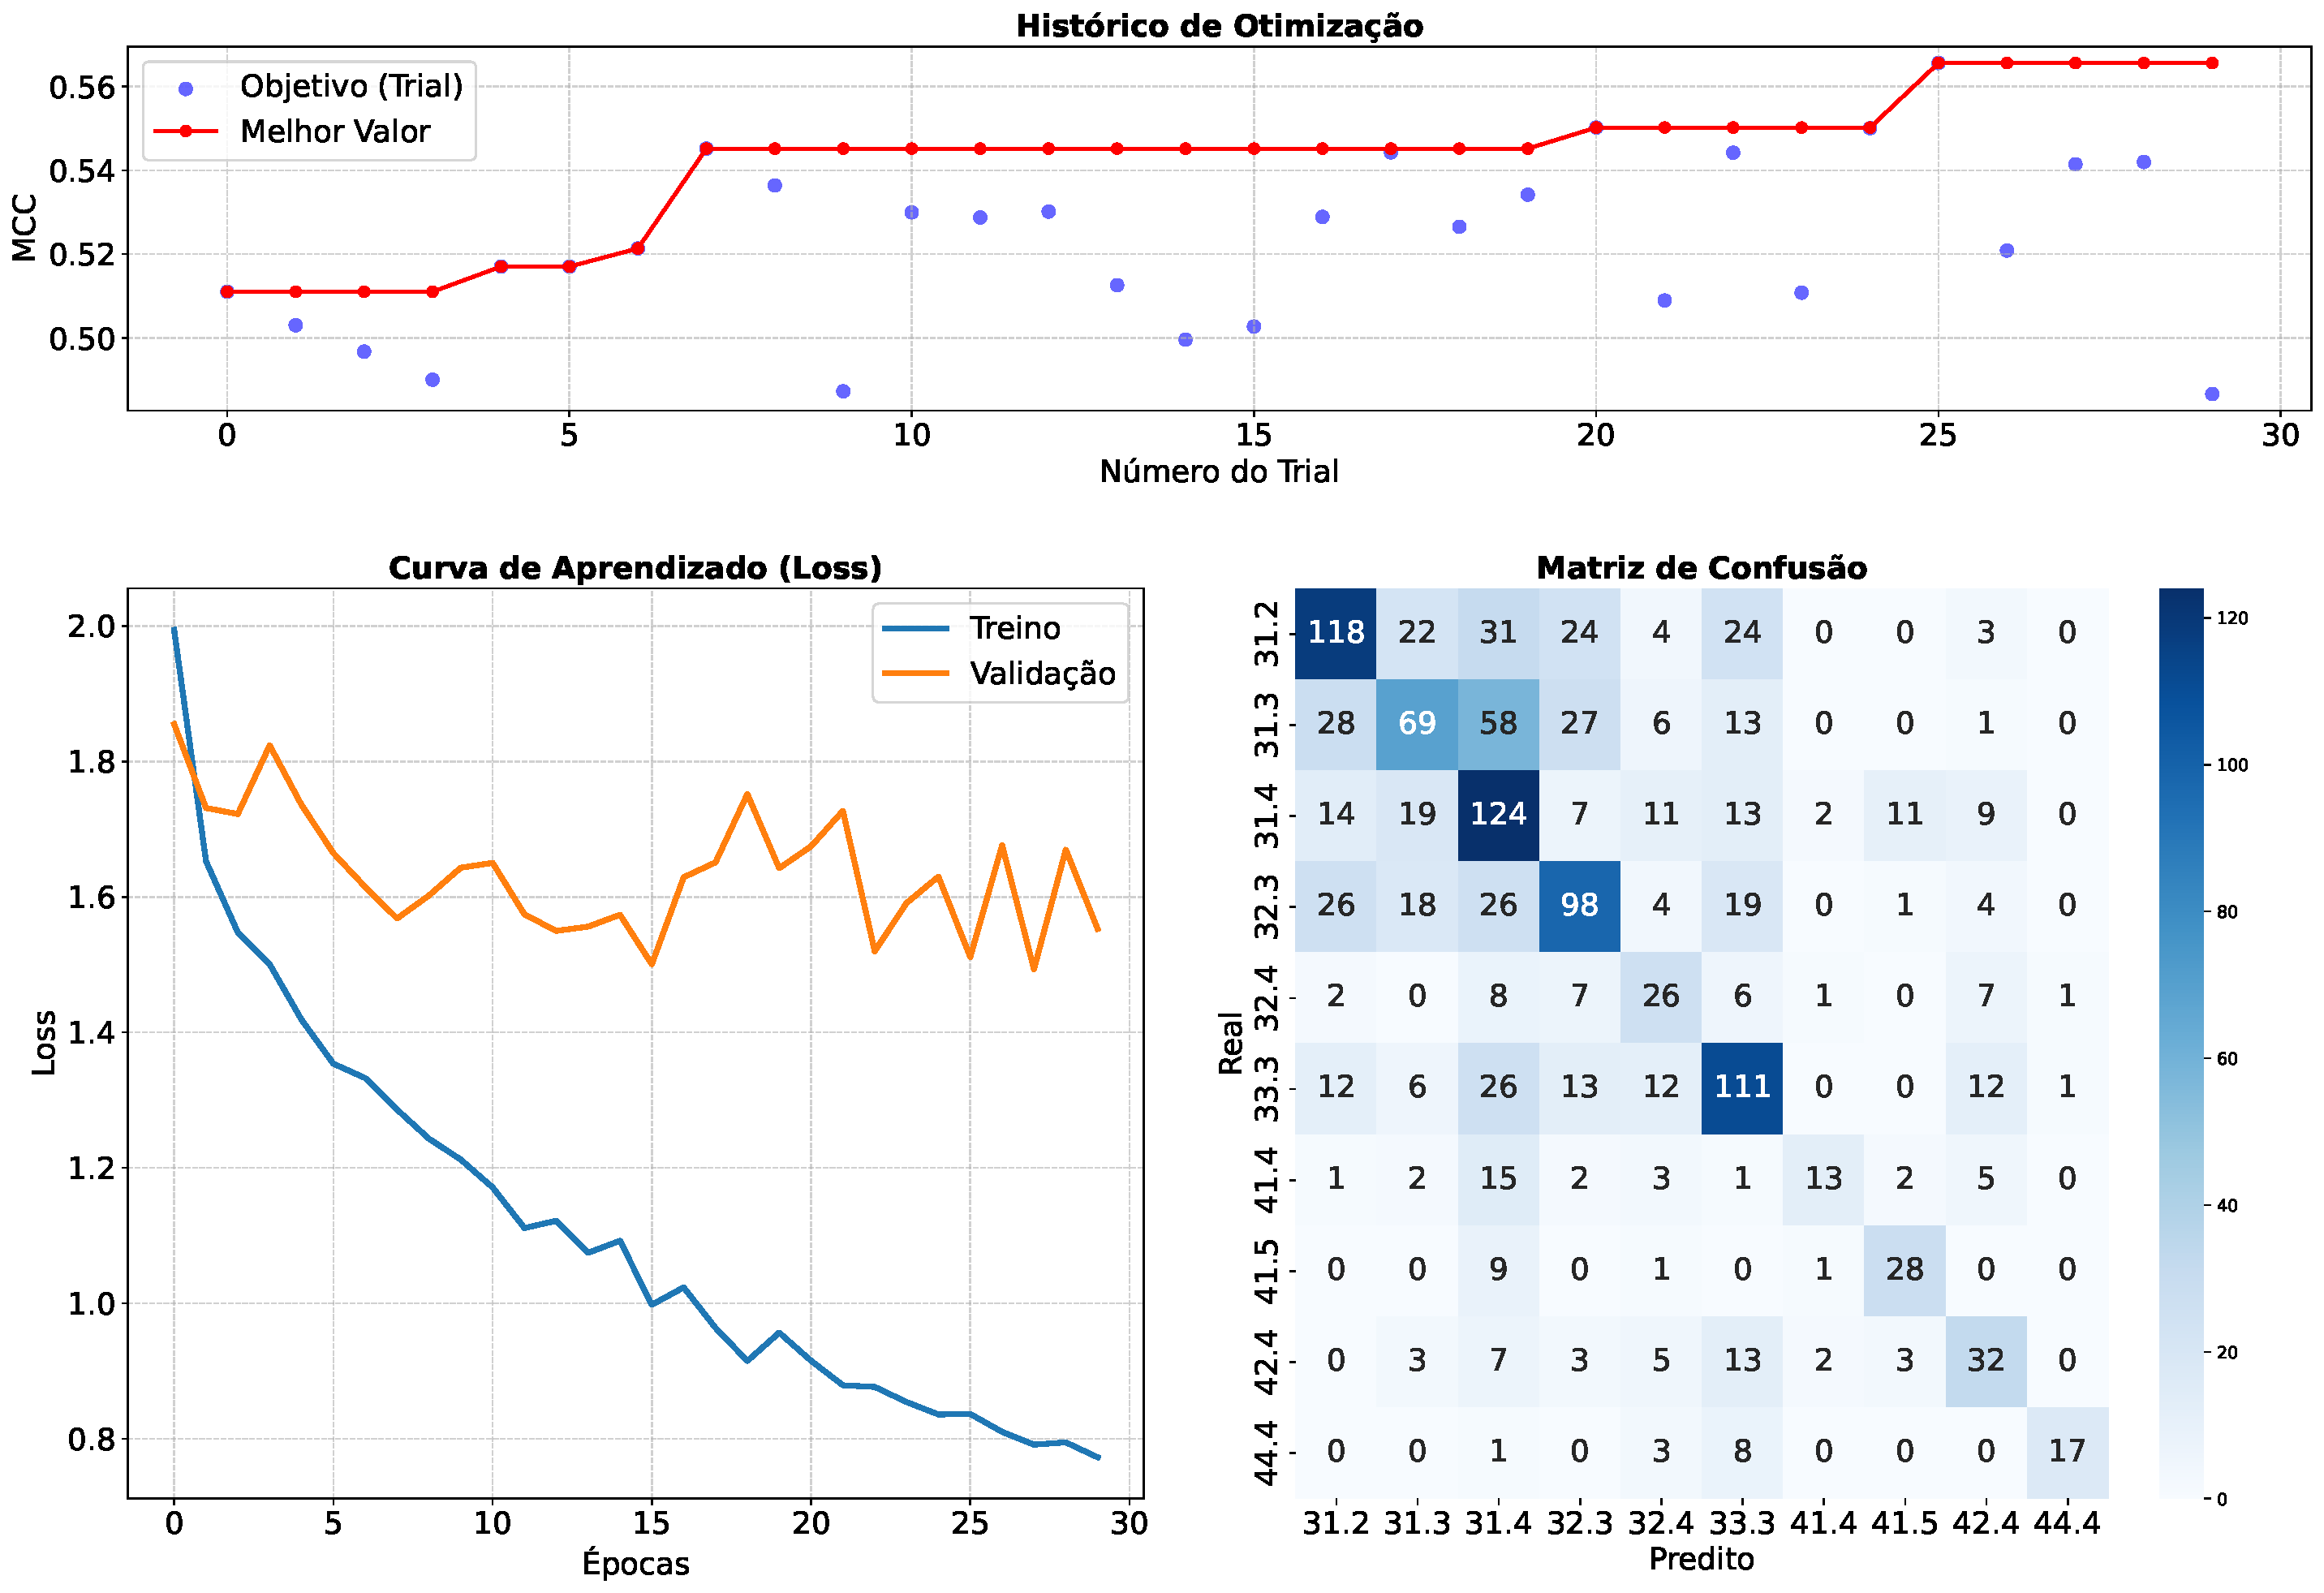
\includegraphics[width=0.9\textwidth]{tex/appendix/experiments/swin_v1_AB_opt_aug/dashboard_consolidado.pdf}
        \caption{Histórico de Otimização, Curvas de Aprendizado e Matriz de Confusão - swin\_v1\_AB\_opt\_aug}
    \end{figure}
\end{minipage}

\clearpage
\pdfpagewidth=297mm \pdfpageheight=210mm
\newgeometry{left=1.5cm, right=1.5cm, top=2.5cm, bottom=2cm} 
\begin{figure}[H]
    \centering
    \makebox[\textwidth][l]{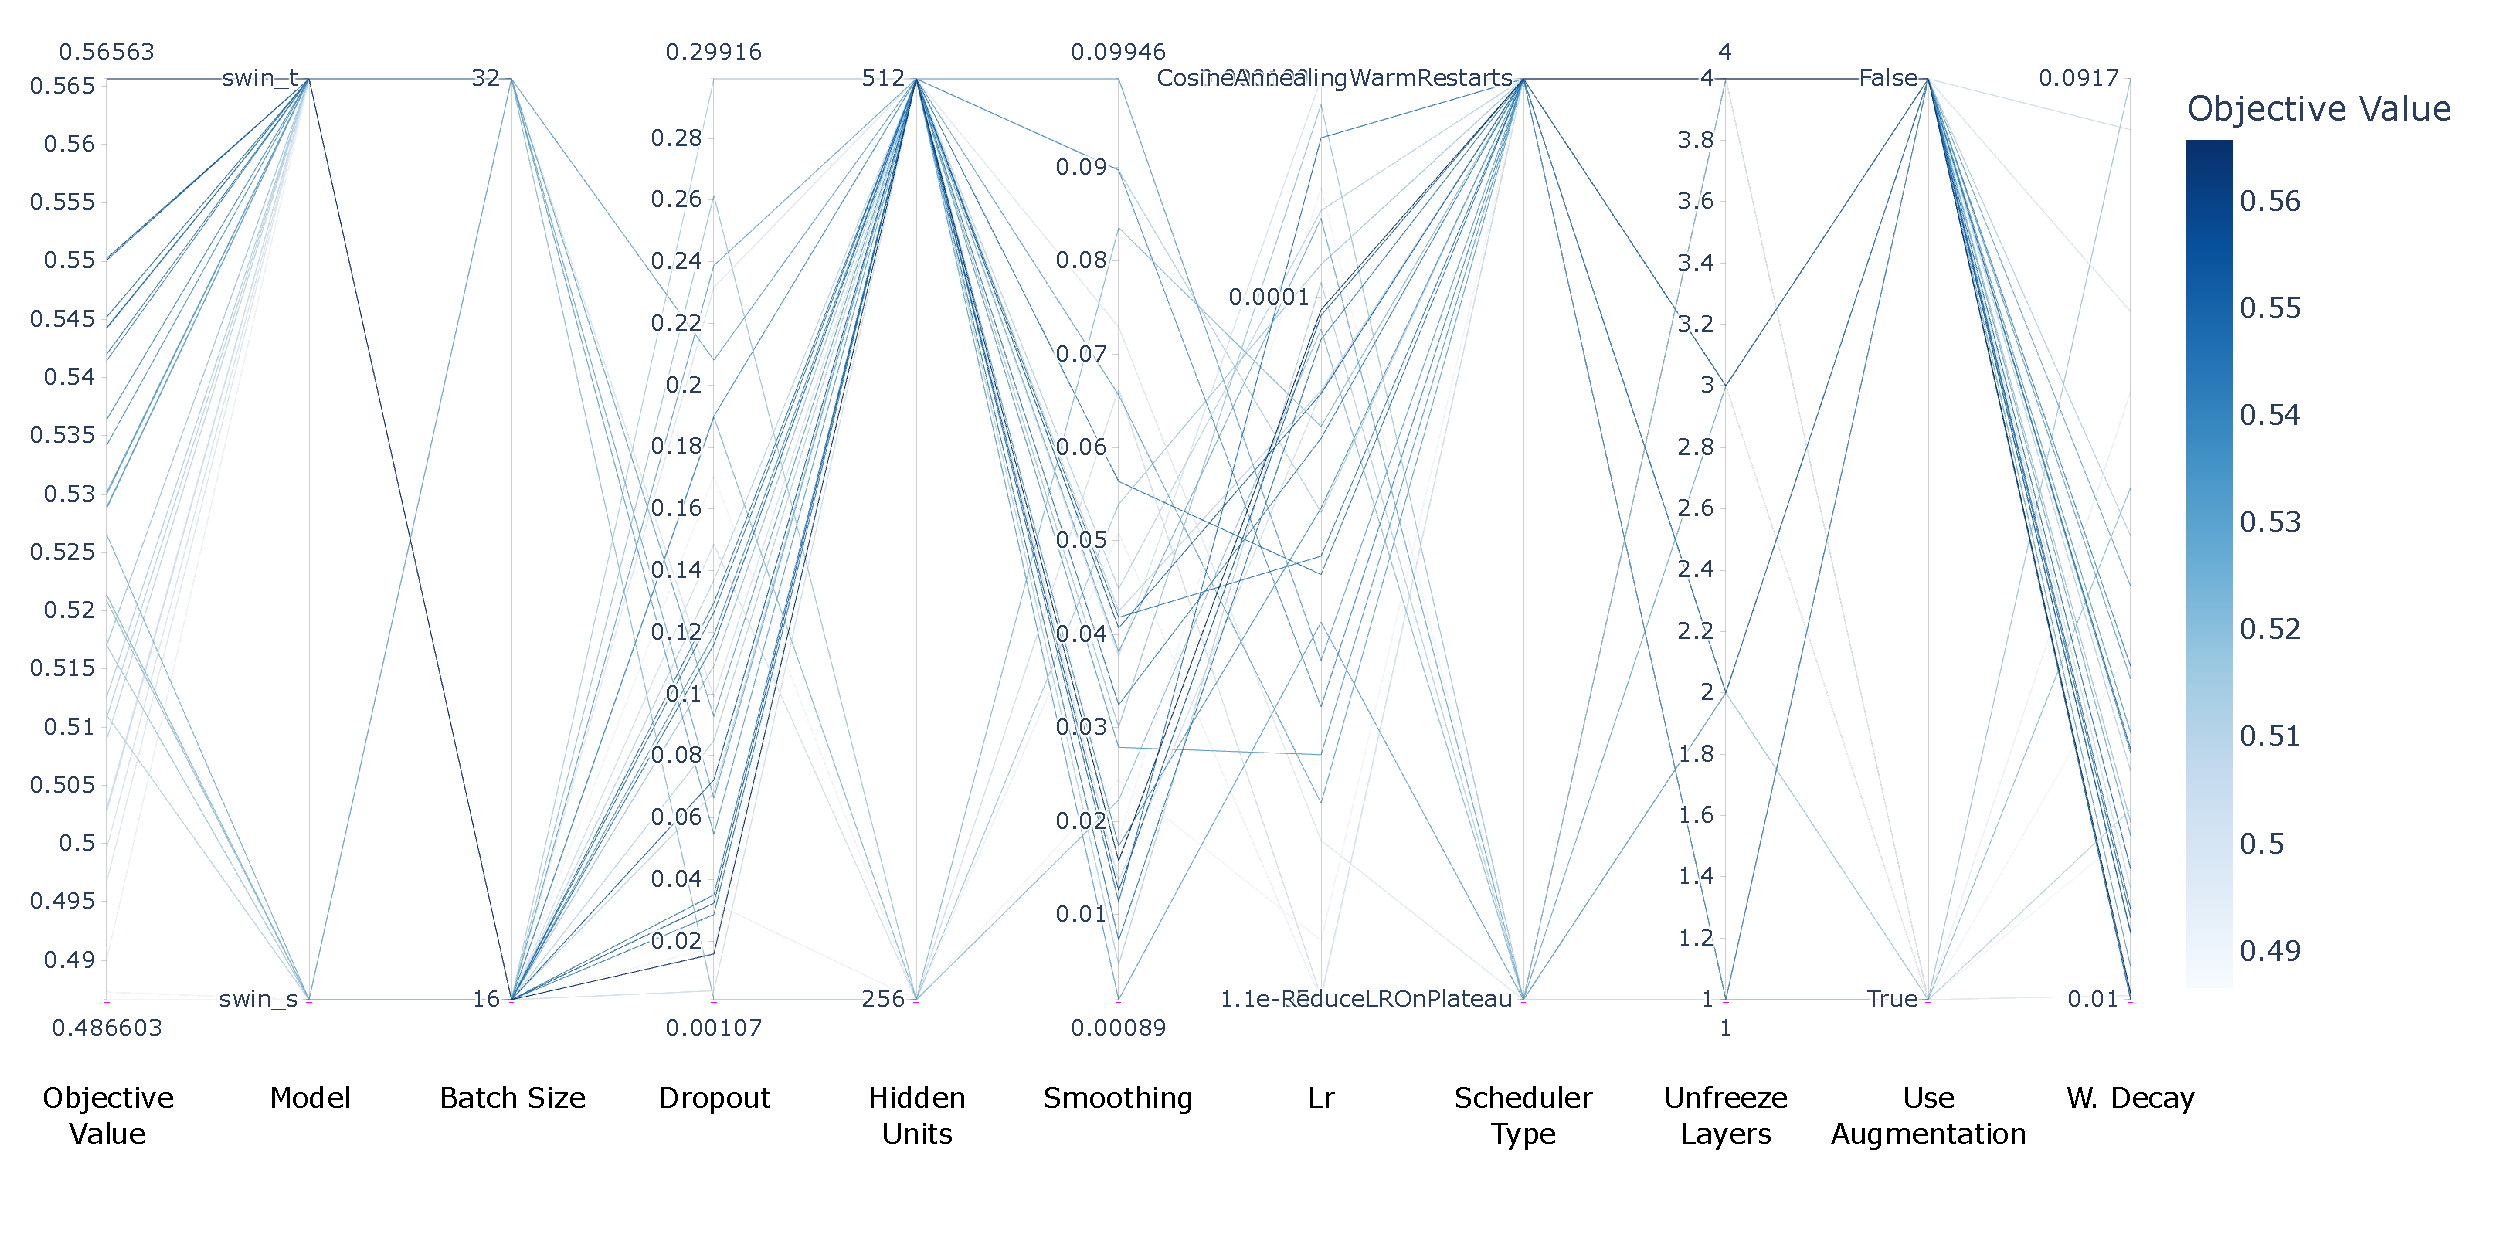
\includegraphics[width=1.7\textwidth]{tex/appendix/experiments/swin_v1_AB_opt_aug/optuna_parallel.pdf}}
    \caption{Coordenadas Paralelas dos principais hiperparâmetros para swin\_v1\_AB\_opt\_aug}
\end{figure}
\clearpage
\pdfpagewidth=210mm \pdfpageheight=297mm
\restoregeometry
\newpage
